\chapter{Mapy}

\begin{figure}[h]
\begin{centering}
\includegraphics[width=1\textwidth]{obrazky/mapa-horiz_w}\label{fig:mapa-mlynov}
\par\end{centering}

\protect\caption{Mapa Mlynskej doliny}
\end{figure}

% TODO!!! dorobit pavilon S - DONE
\begin{figure}[h]
	\begin{centering}
		\vspace{-0.6cm}
		\includegraphics[width=1\textwidth]{obrazky/plan_matfyzu}\label{fig:mapa_fmfi}
		\par\end{centering}
	
	
	\protect\caption{Mapa FMFI}
	Online interaktívnu mapu aj s vyhľadávaním nájdeš na~\href{http://mapa.matfyzjein.sk}{\texttt{mapa.matfyzjein.sk}}, pre smartfóny s Androidom je k dispozícii v Google Play aplikácia ,,Sprievodca FMFI". Okrem označenia jednotlivých miestností (a kto v nej sedí), navigácie ,,z-do" v nej nájdeš aj denné menu v jedálňach.
\end{figure}

\begin{figure}[h!]
	\begin{centering}
		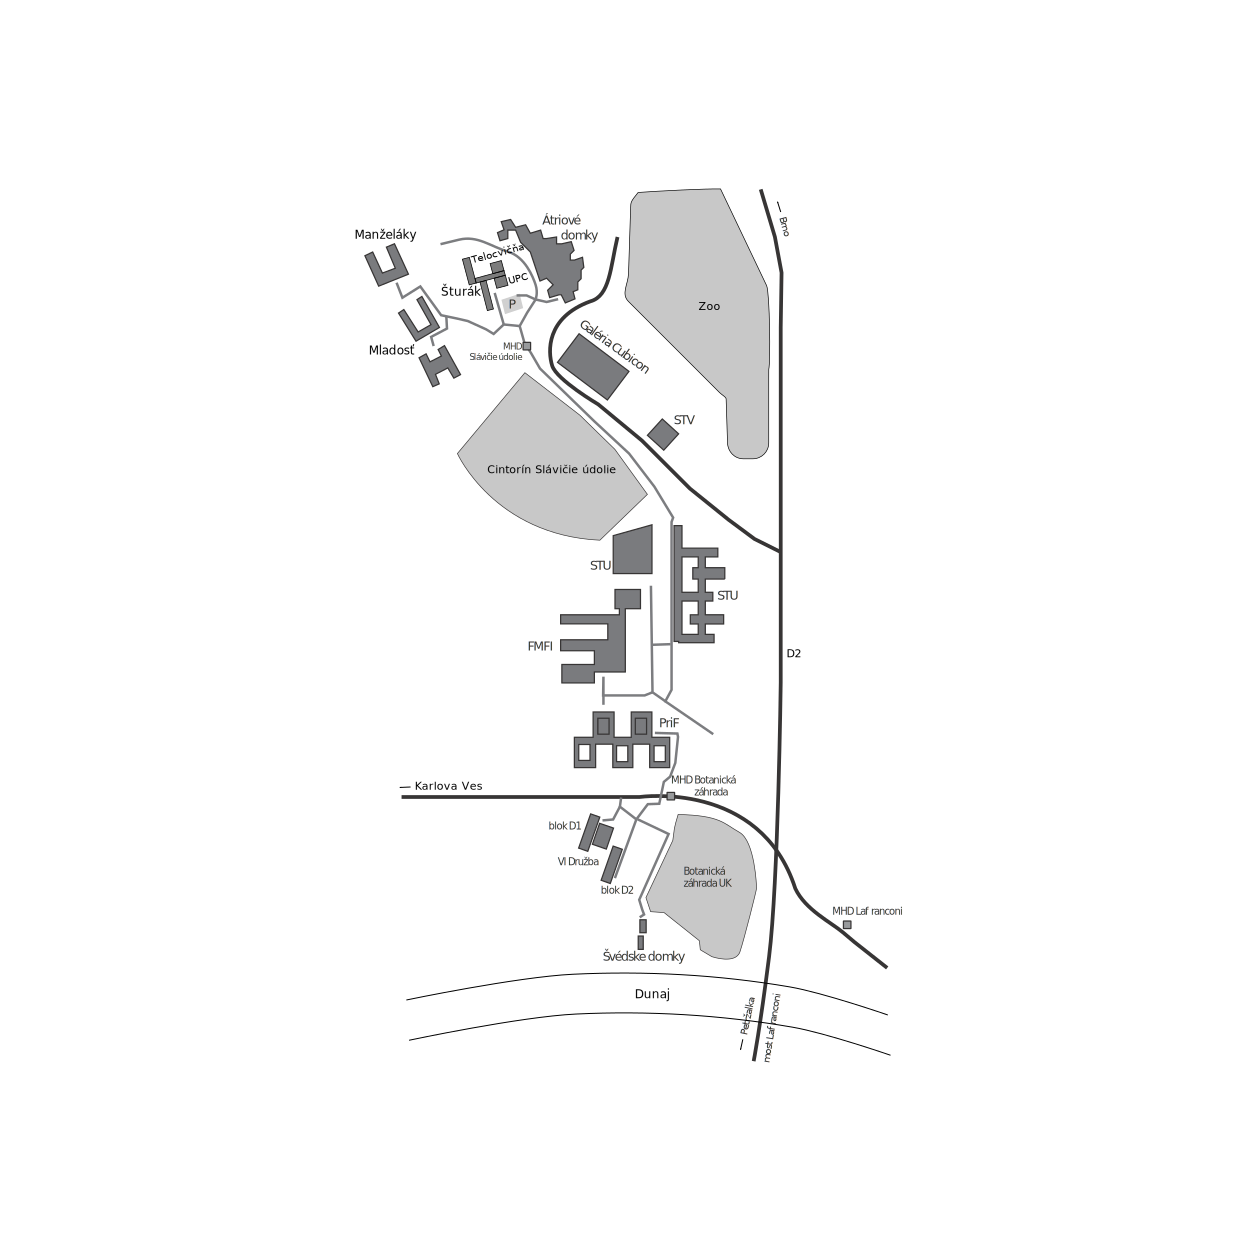
\includegraphics[width=1.8\textwidth,height=1.059\textheight,keepaspectratio]{obrazky/mapka_okolie_PriF}\label{fig:mapka_okolia_PriF}
		\par\end{centering}
	\protect\caption{Mapa širšieho okolia Mlynskej doliny}
\end{figure}




